\subsection{X-Means}
\subsubsection{Hyper-parameters}
We have explored the effect of the main hyper-parameter of the X-Means, which is the maximum number of clusters. The results have varied significantly for the different datasets. The results and plots presented here show the number of clusters predicted by the X-Means algorithm (red points) and their averaged value (blue line) over a range of maximum clusters. Each configuration has been run several times to reduce the effects of the stochastic nature of the algorithm.

\begin{enumerate}
    \item \textbf{Hepatitis:}
    \\ When analyzing the effect of increasing the maximum number of clusters when processing the hepatitis dataset, we can observe that the algorithm converges to 2 clusters and thus the mean number of predicted clusters does not vary significantly when testing in a range from 2 to 10 for the maximum number of clusters parameter, with the exception of a few runs where the algorithm found 3 clusters.
    \begin{figure}[H]
        \centering
        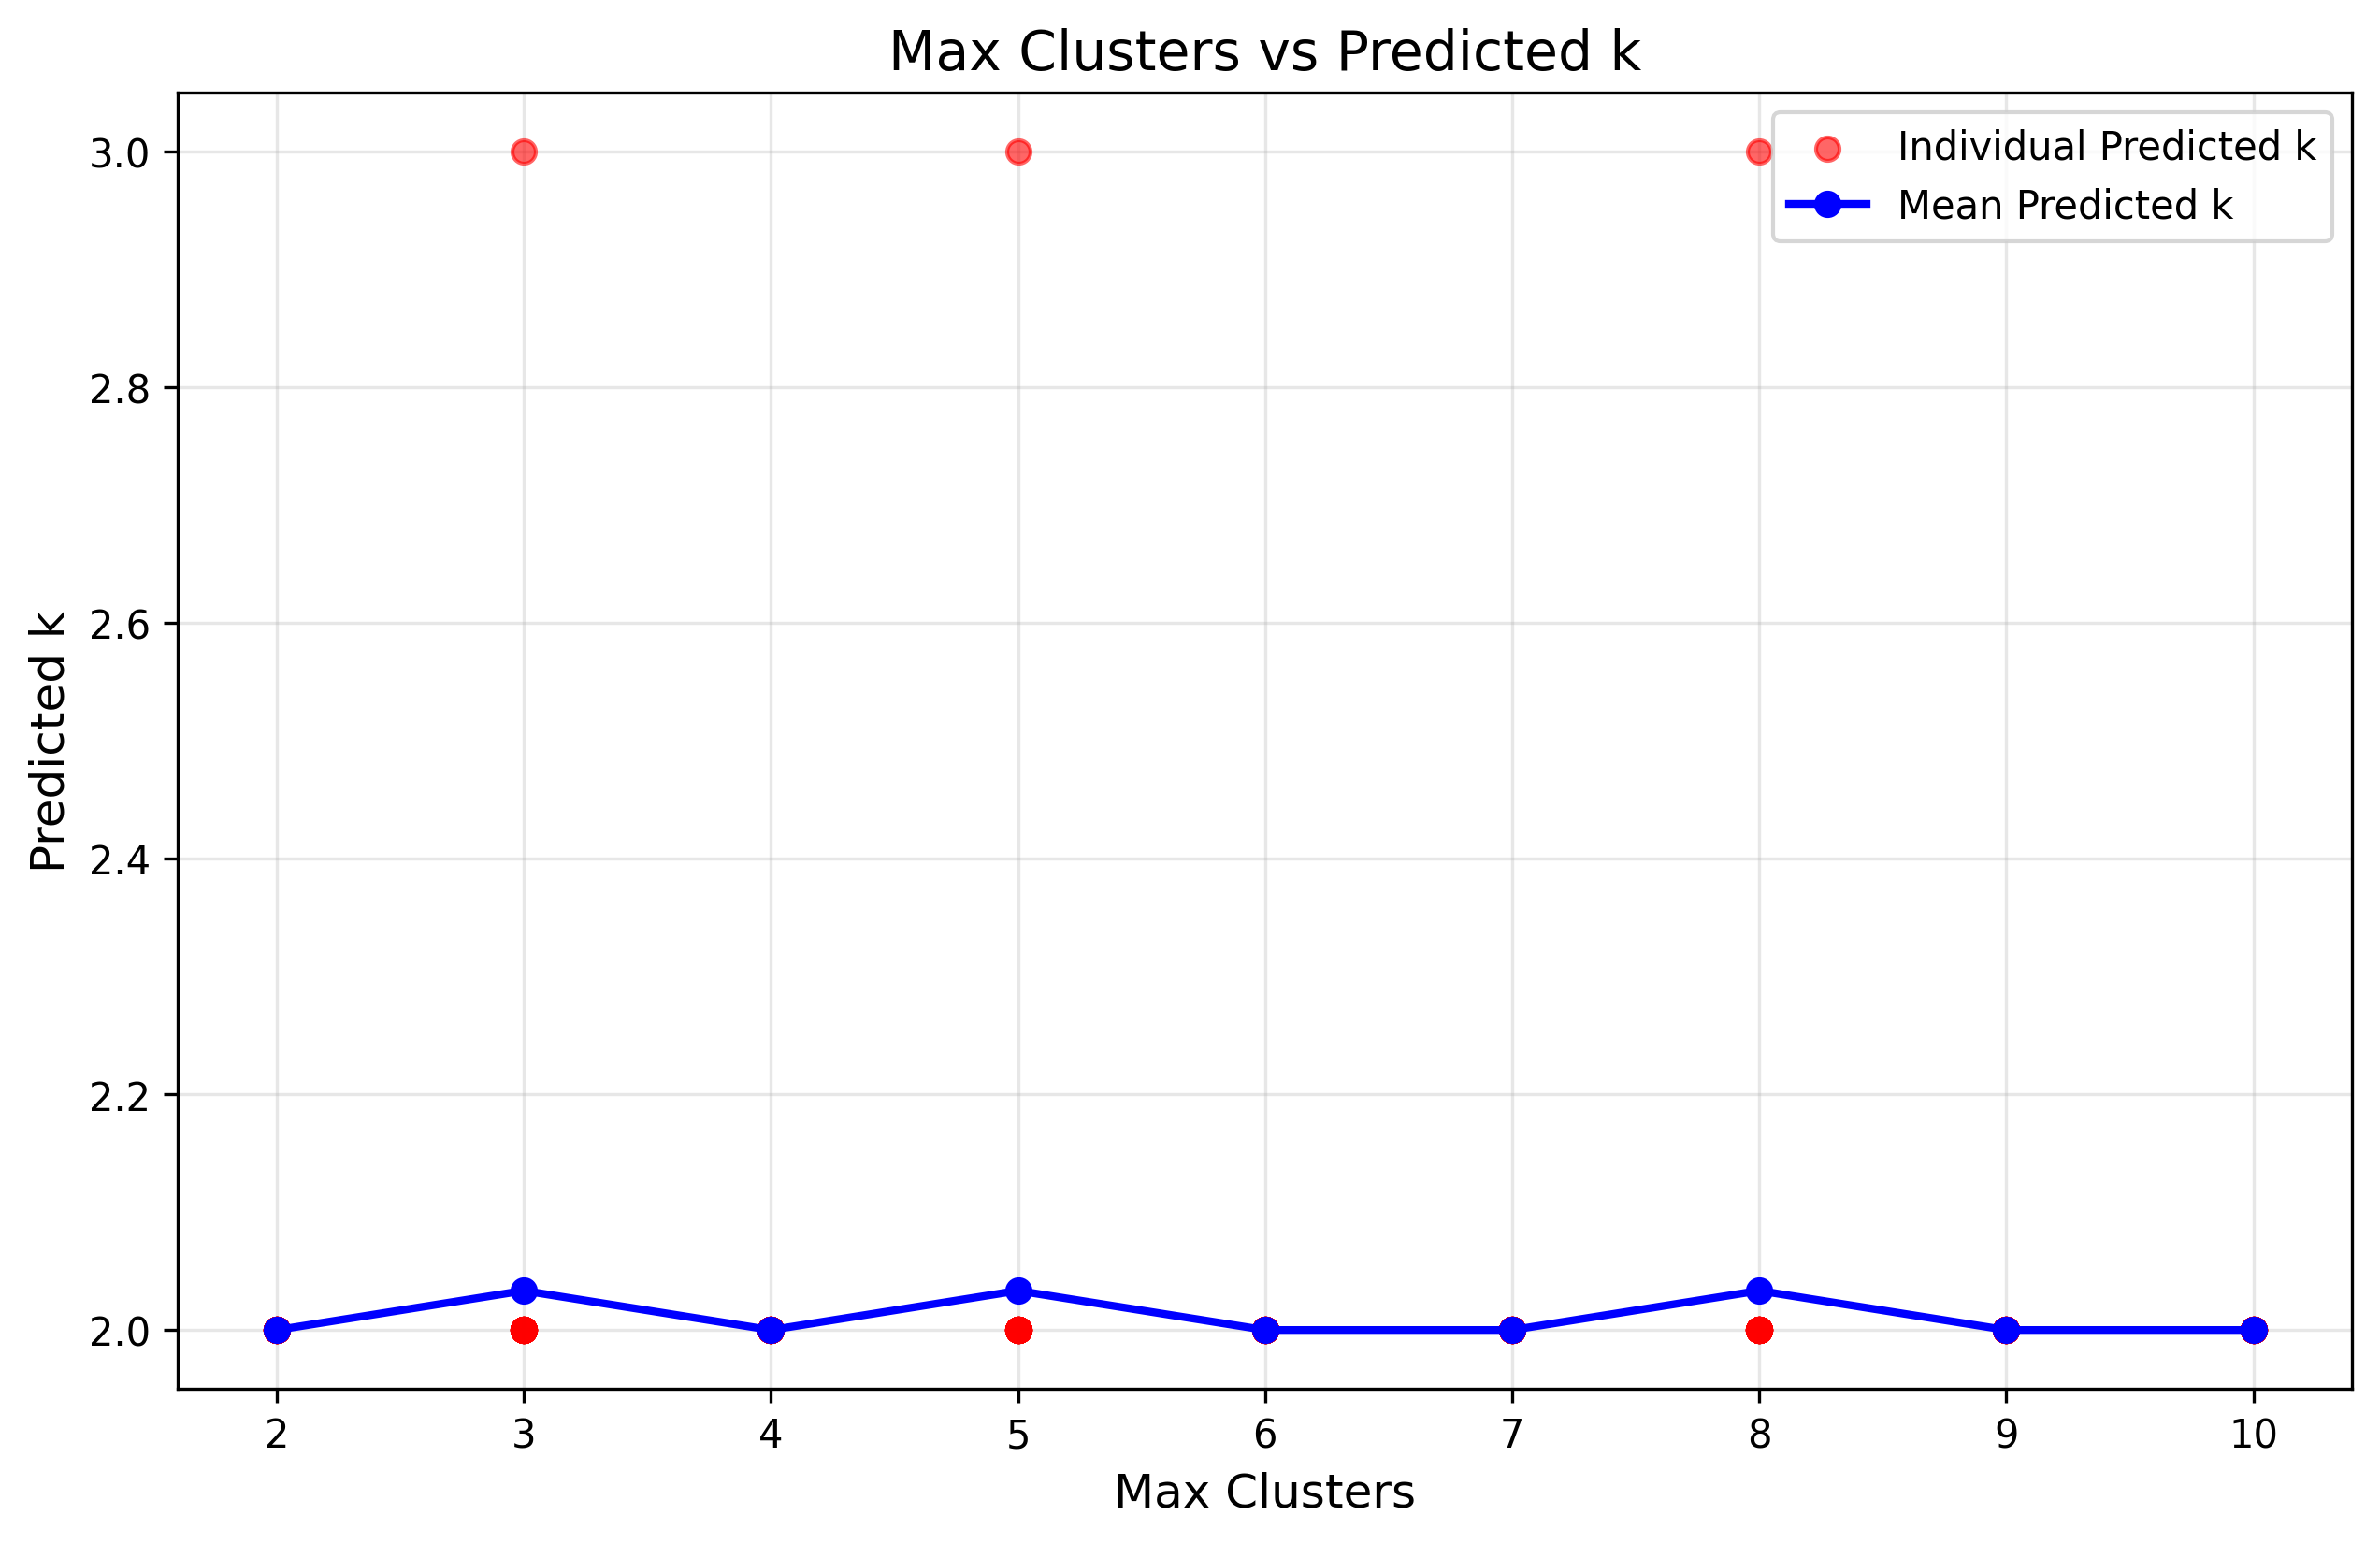
\includegraphics[width=0.7\linewidth]{figures/XMeans/hepatitis_max_k_vs_predicted_k.png}
        \caption{Max number of clusters vs predicted number of clusters (hepatitis dataset)}
    \end{figure}
    \item \textbf{Mushroom:}
    \\ The results for the mushroom dataset are quite different from the ones obtained in hepatitis. For this experiment each configuration was run 10 times. The plot shows clearly how the runs with a maximum number of clusters lower than 600 always finished with the maximum number of clusters. When the maximum number of clusters was higher than 600 the algorithm would repeatedly converge to a predicted number of clusters lower than the maximum, with this effect being particularly noticeable when plotting the average number of predicted clusters (blue line).
    \begin{figure}[H]
        \centering
        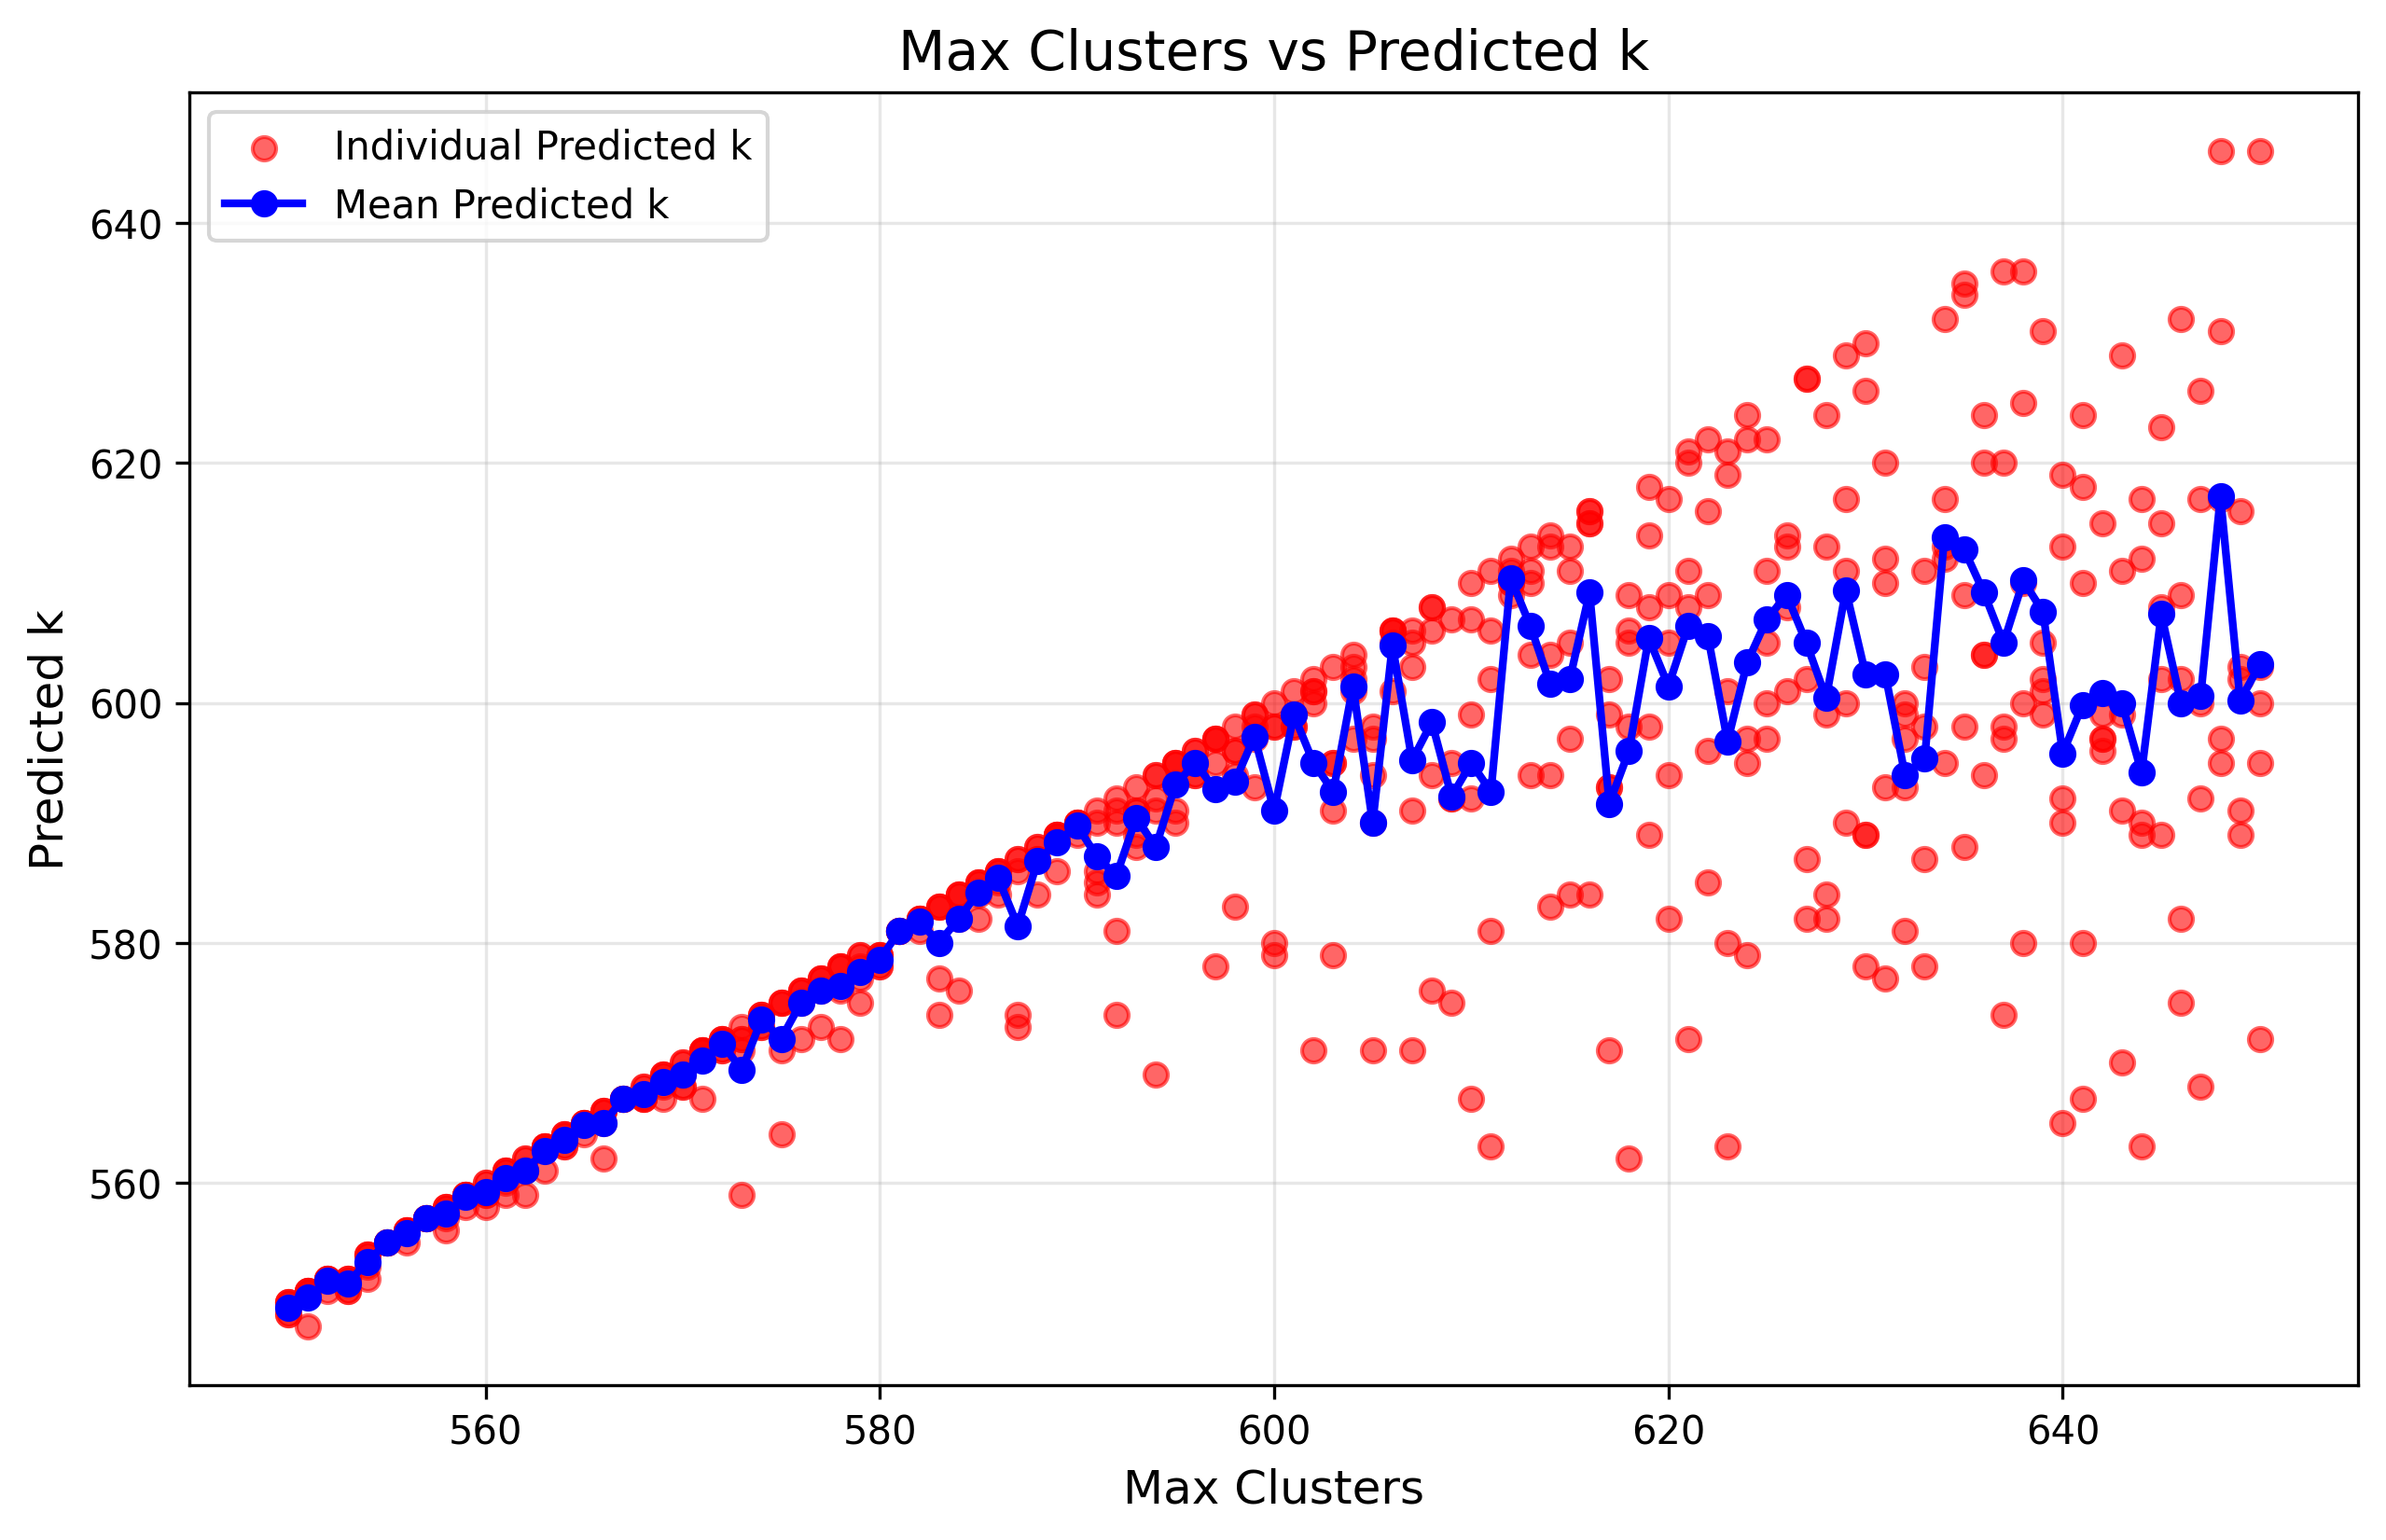
\includegraphics[width=0.7\linewidth]{figures/XMeans/mushroom_max_k_vs_predicted_k.png}
        \caption{Max number of clusters vs predicted number of clusters (mushroom dataset)}
    \end{figure}
    \item \textbf{Pen-based:}
    \\ The analysis of the effects of varying the maximum number of clusters when processing the pen-based dataset are similar to the ones obtained in mushroom, with the difference that here the algorithm converges to a lower number of clusters, around 200 (see figure).
    \begin{figure}[H]
        \centering
        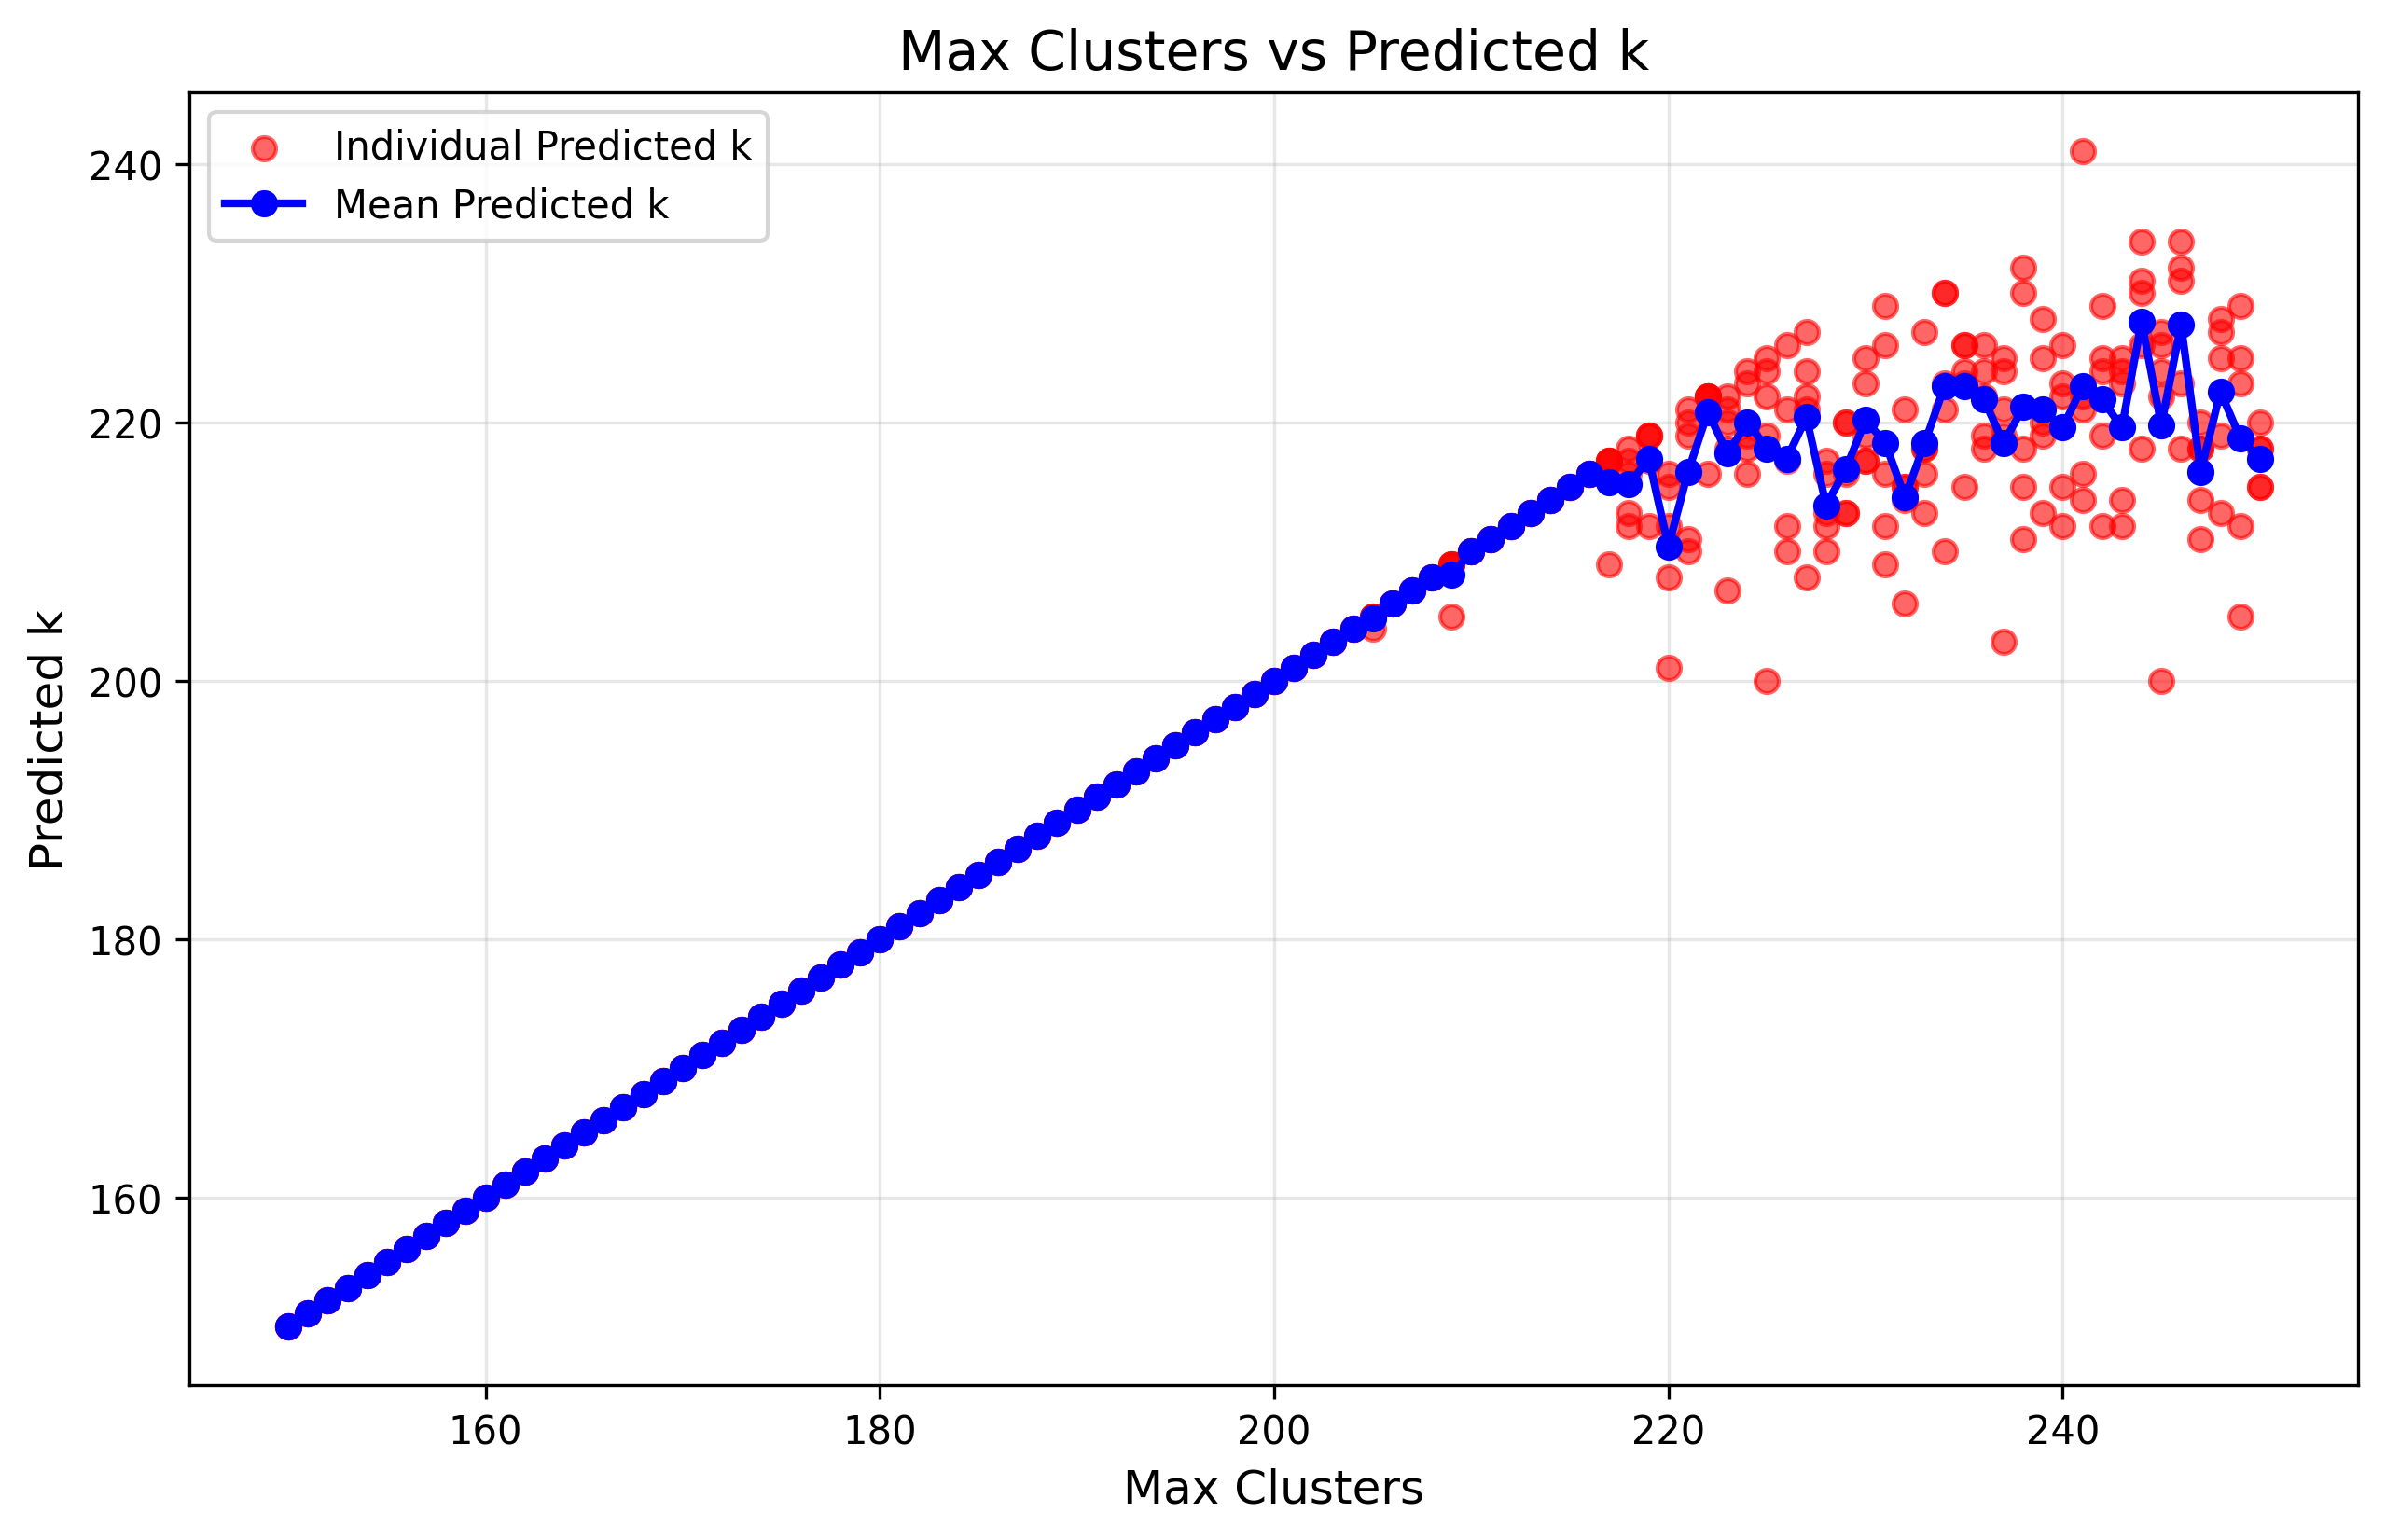
\includegraphics[width=0.7\linewidth]{figures/XMeans/pen-based_max_k_vs_predicted_k.png}
        \caption{Max number of clusters vs predicted number of clusters (pen-based dataset}
    \end{figure}
\end{enumerate}

\subsubsection{Visualization}

Since the datasets we have chosen for this assignment have high dimensionality we have opted for doing Principal Component Analysis (PCA) to be able to plot the points and the predicted clusters. 

For the hepatitis dataset, the fewer samples and the fact that the X-Means converged to a lower number of clusters allows us to easily plot it using the first two principal components. Both the mushroom and pen-based datasets are easier to explore using an interactive 3D plot.

\begin{enumerate}
    \item \textbf{Hepatitis:}
        \\\\Plotting the points in the hepatitis dataset using the first two principal components we can observe how the points have been clustered divided in the middle.
        \begin{figure}[H]
            \centering
            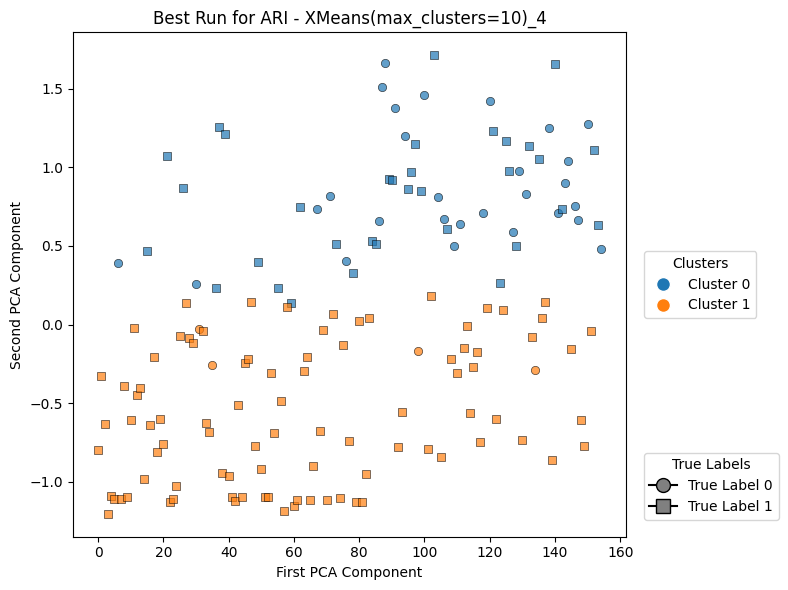
\includegraphics[width=0.7\linewidth]{figures/XMeans/hepatitis_visualization.png}
            \caption{Hepatitis dataset 2D visualization}
        \end{figure}
    \item \textbf{Mushroom:}
        \\\\The plot of the mushroom dataset helps us understand why the X-Means has converged to such a high number of clusters, when seen from the distance the points seem to form few elongated clusters, however, zooming in we can observe how the big clusters are formed by smaller, clearly separated clusters.
        \begin{figure}[H]
        \centering
        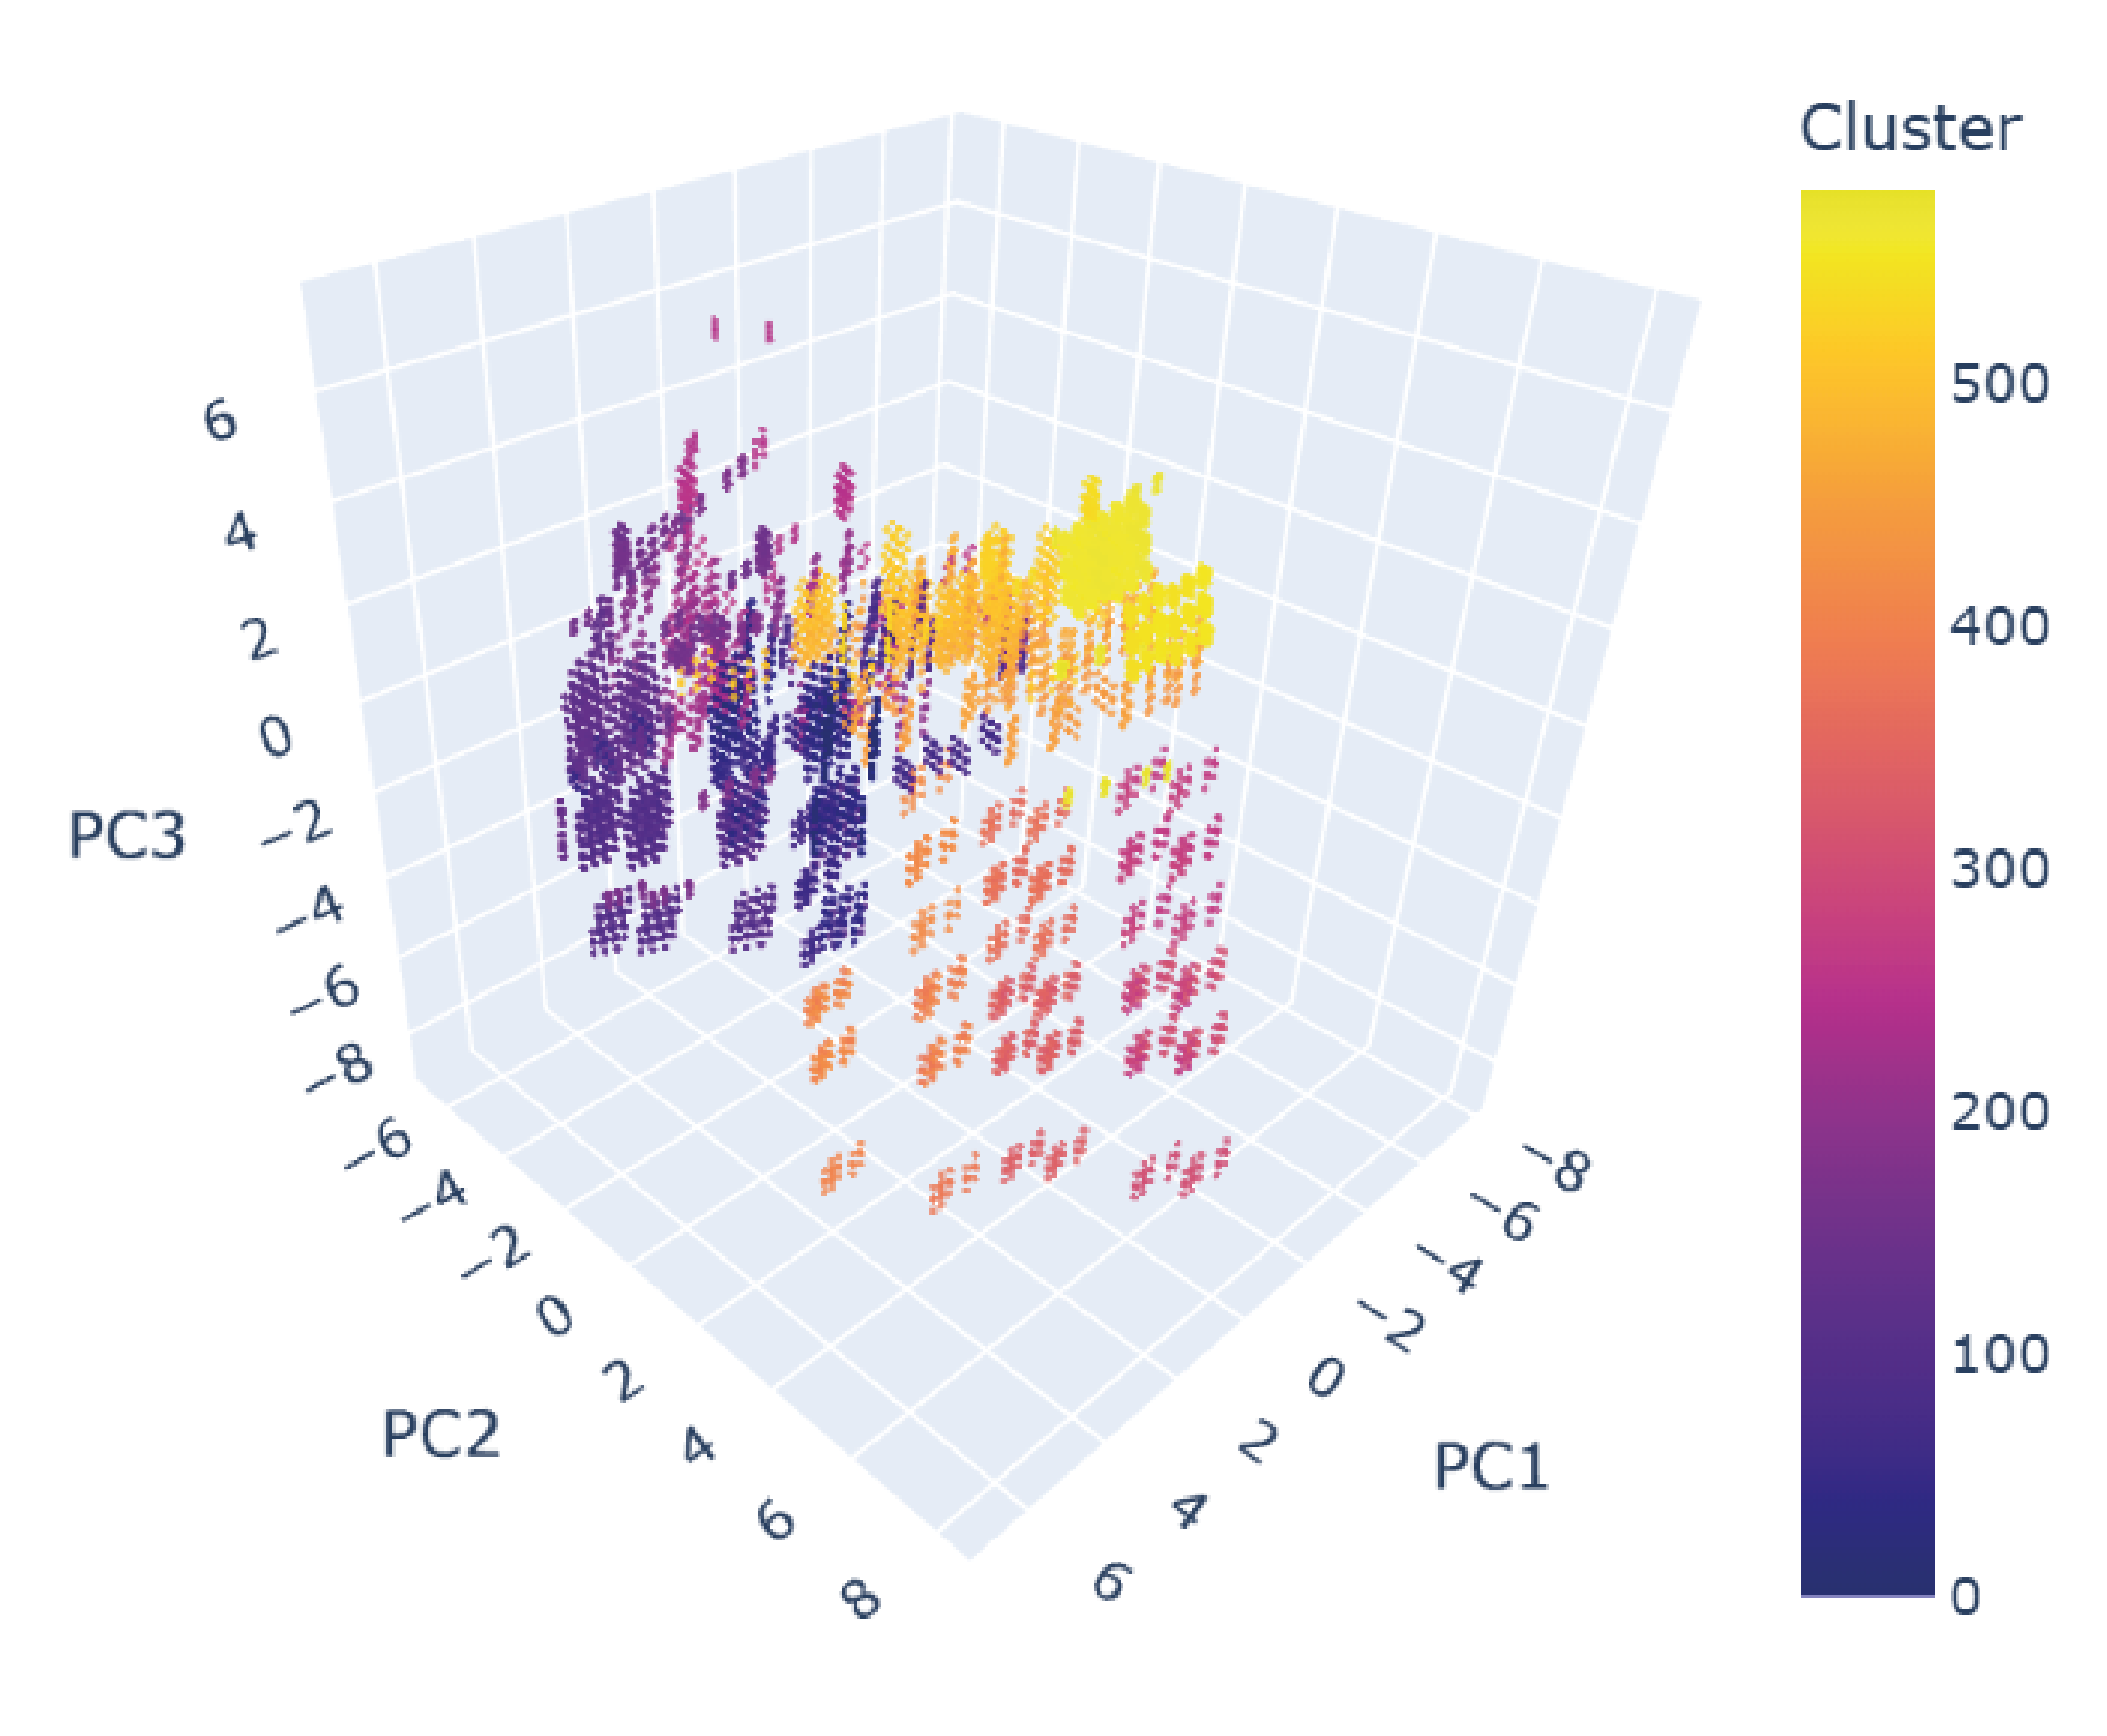
\includegraphics[width=0.7\linewidth]{igures/XMeans/mushroom_visualization.png}
        \caption{Mushroom dataset 3D visualization}
        \end{figure}
    \item \textbf{Pen-based} 
    \\\\ Similarly to the visualization of the mushroom dataset, visualizing the pen-based dataset in 3D helps us understand how the algorithm has clustered the data, with big clusters formed by smaller ones.
    \begin{figure}[H]
    \centering
    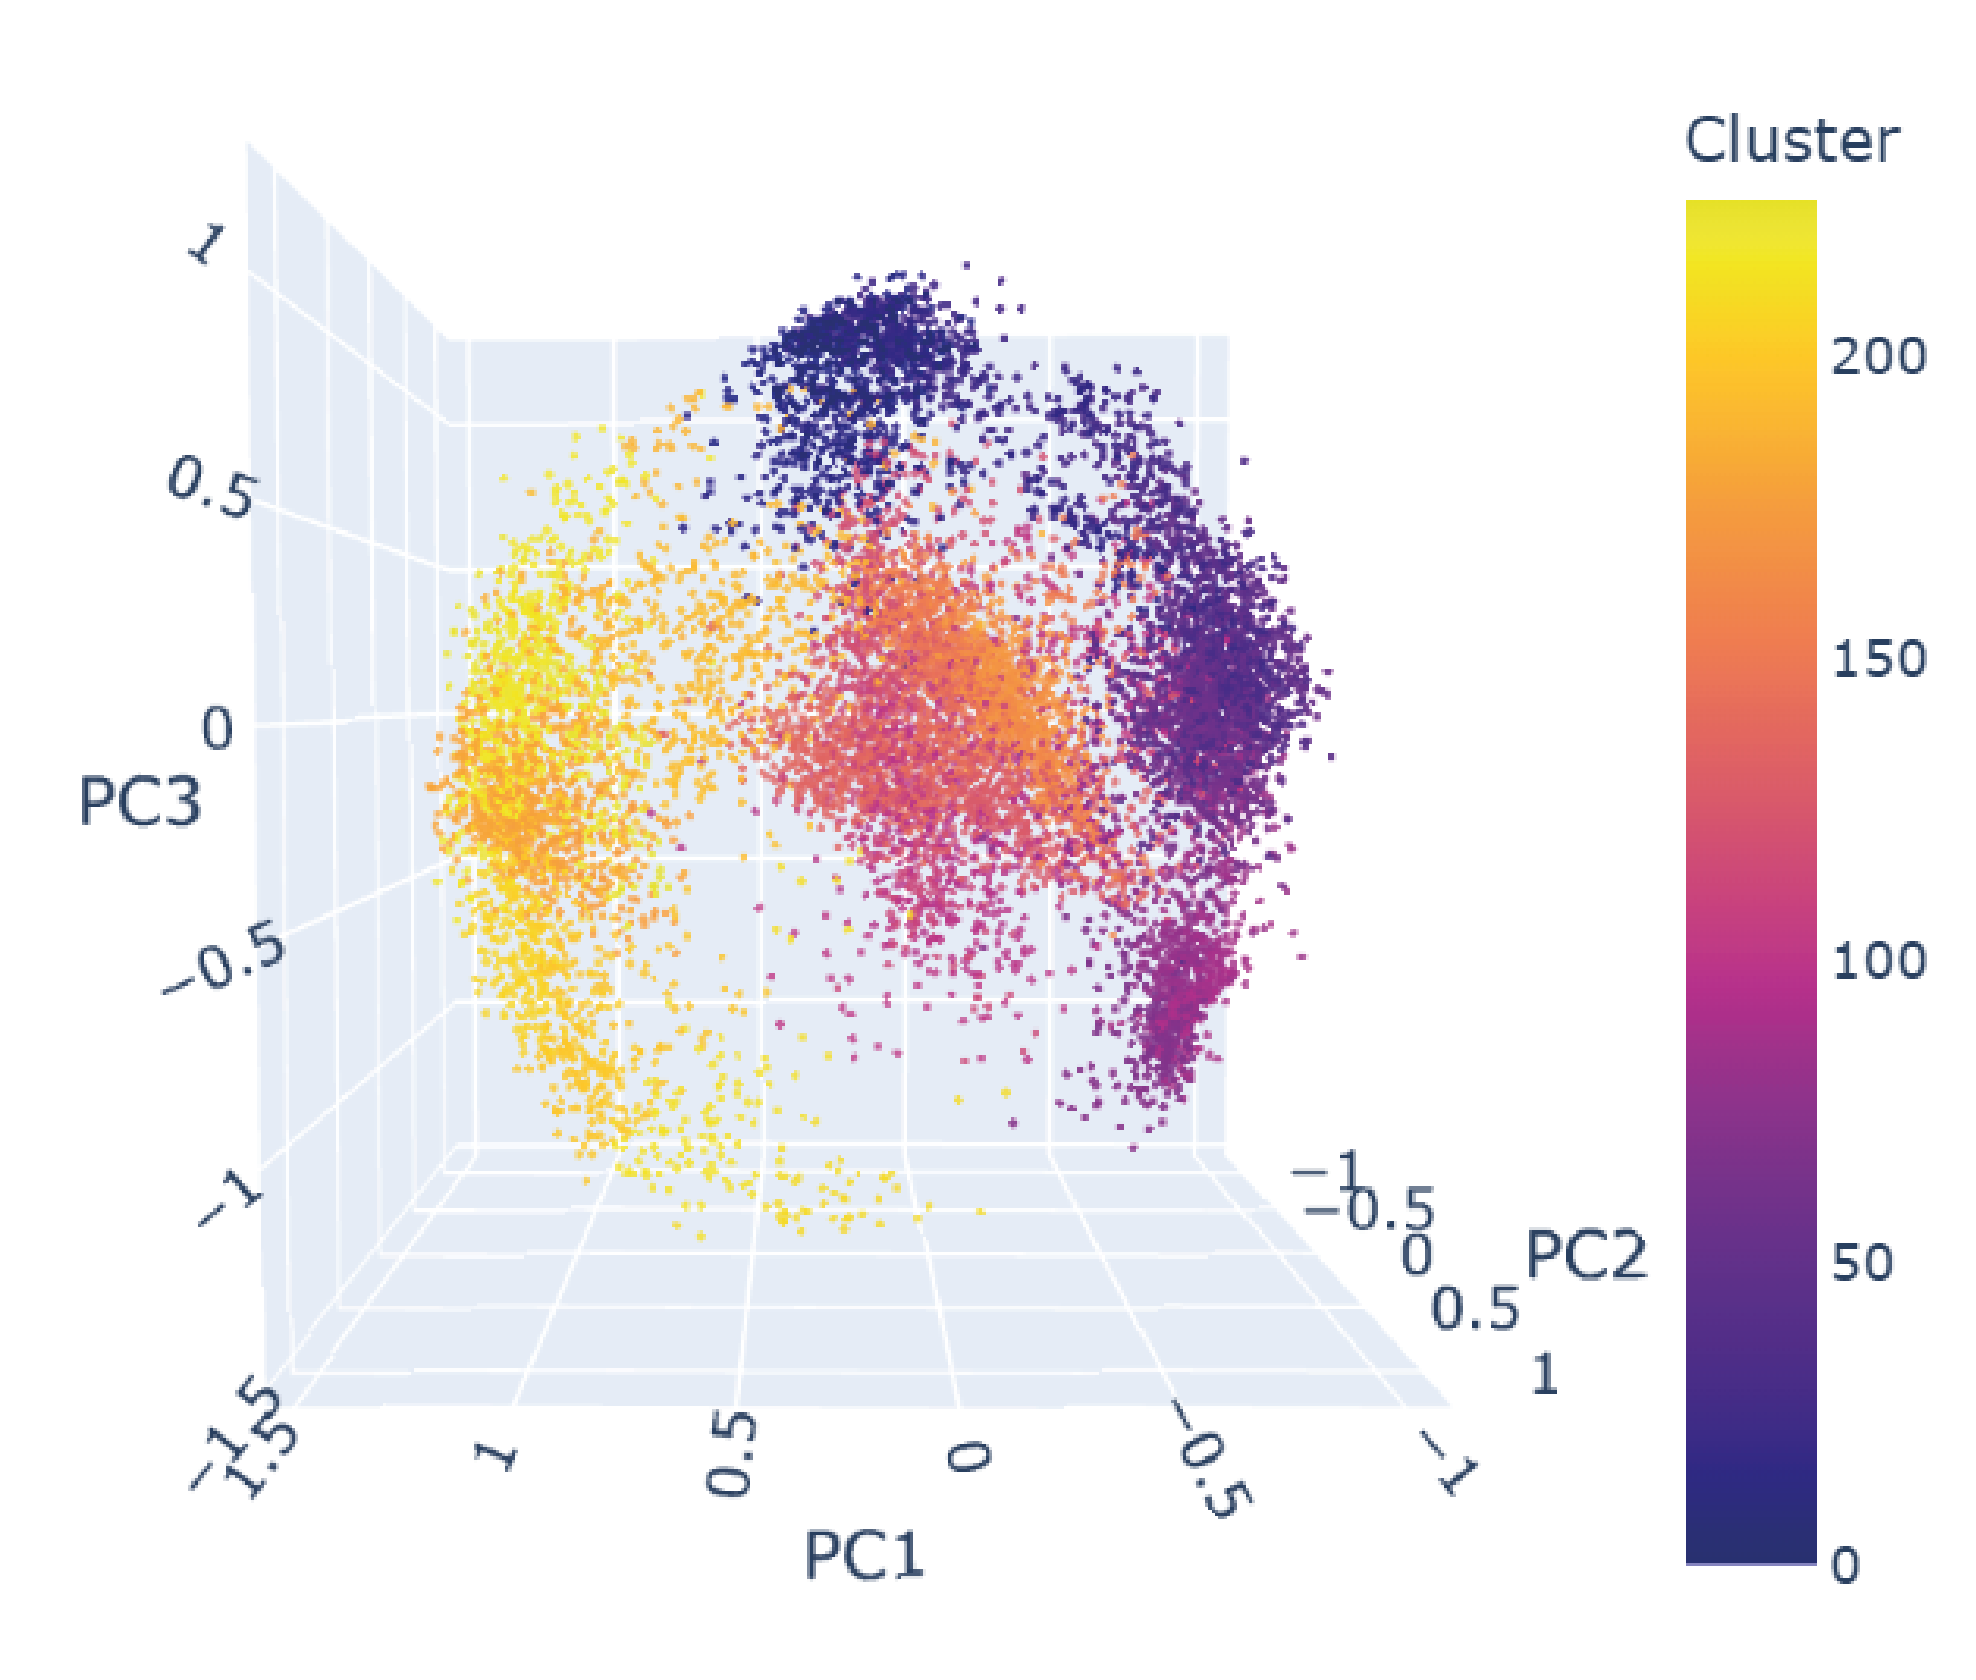
\includegraphics[width=0.7\linewidth]{igures/XMeans/pen-based_visualization.png}
    \caption{Pen-based dataset 3D visualization}
\end{figure}

\end{enumerate}